\documentclass{report}

% Basic packages and settings
\usepackage{xcolor}
\usepackage{ulem}
\usepackage{indentfirst}
  \setlength{\parindent}{2.5em}
\setlength{\lineskiplimit}{3pt}
\setlength{\lineskip}{3pt}
\usepackage{geometry}
  \geometry{top = 0.8in, bottom = 1in}
\usepackage{graphicx}
  \graphicspath{{./mpl-image/}}

% My newcommand & newenvironment
\newcommand{\pkg}[1]{\texttt{#1}}
  \newcommand{\Py}{\pkg{Python}}
  \newcommand{\NumPy}{\pkg{NumPy}}
  \newcommand{\SciPy}{\pkg{SciPy}}
\newcommand{\mpl}{\texttt{Matplotlib}}
\newcommand{\Emph}[1]{\textcolor{cyan!80!white}{{\bfseries #1}}}
\newcommand{\nextblock}{\vspace{2ex}}

% List settings
\usepackage{enumitem}
  \setlist[enumerate]
    {font=\bfseries,labelindent=0pt,itemsep=0pt,parsep=0pt,topsep=1ex,partopsep=0pt}
  \setlist[itemize]
    {font=\bfseries,itemsep=0pt,parsep=0pt,topsep=1ex,partopsep=0pt}
  \setlist[description]
    {font=\bfseries\ttfamily,itemsep=0pt,parsep=0pt,topsep=1ex,partopsep=0pt}

% Code
\usepackage{tcolorbox}
  \tcbuselibrary{listings,skins,breakable}
% Avoid copy line numbers of the listing code
\usepackage{accsupp}
	\newcommand{\emptyaccsupp}[1]{\BeginAccSupp{ActualText={}}#1\EndAccSupp{}}
% Code-only Environment
\newtcblisting{py}{breakable,skin=bicolor,colback=gray!30!white,
  colbacklower=white,colframe=cyan!75!black,listing only, 
  left=6mm,top=2pt,bottom=2pt,
  % listing style
  listing options={language=Python,basicstyle=\small\ttfamily,
  keywordstyle=\color{blue},commentstyle=\color{green!50!black},
  numbers=left,numberstyle=\tiny\color{red!75!black}\emptyaccsupp,
  emptylines=1,escapeinside=``}}
% Inline Python commands
\newtcbox{\python}[1][green]{on line,before upper=\ttfamily,
  arc=0pt,outer arc=0pt,colback=#1!10!white,colframe=#1!50!black,
  boxsep=0pt,left=1pt,right=1pt,top=1pt,bottom=1pt,
  boxrule=0pt,bottomrule=1pt,toprule=1pt}

% Hyperref
\usepackage{hyperref}
\hypersetup{colorlinks, bookmarksopen = true, bookmarksnumbered = true, pdftitle=Python-matplotlib, pdfauthor=K.L Wu, pdfstartview=FitH}

% Cover of Report
\title{Simple \mpl}
\author{K.L Wu}
\date{Last revision: \today}

\begin{document}

\maketitle

\chapter{Introduction}
\mpl\ is a package of \Py\ (\url{https://www.python.org/}) and it provides strong 2D plotting support. Here are some features of it:
\begin{enumerate}
\item It can be used in both \Emph{interactive} and \Emph{non-interactive} mode.
\item It is allowed to export \Emph{raster} or \Emph{vector} images. Supporting formats include: PNG, JPG, BMP (Raster); EPS, SVG, TIFF, PDF (Vector).
\item Similar syntax with MATLAB, but might have better visualization performance.
\item It's integrated with \LaTeX\ markup.
\end{enumerate}

Visit its main website: \url{http://matplotlib.org/} to find more information and sample images of \mpl .

\section{How to get it?}
You can simply install a distribution of \Py, say, Anaconda (\href{https://www.continuum.io/downloads}{Free download here}), to make sure \mpl\ is installed on your computer. 

If you are an advanced \Py\ user, you can also install \mpl package by yourself. Running the setup.py script or downloading unofficial .whl files from \href{http://www.lfd.uci.edu/~gohlke/pythonlibs/#matplotlib}{UC Irvine Unofficial whl \Py\ Downloadpage} and run command line: \texttt{pip install matplotlib.whl} both works.

\section{Dependencies}
You should first install \NumPy\ before getting \mpl .

\NumPy\ is a basic \Py\ module for data works under \Py . It provides high calculation accurancy, many useful predefined math functions, and easier matrices access for \Py\ users. Visit \url{http://www.numpy.org/} for more details.

To check whether you have already had a \NumPy\ installed on your computer, use command line as below:
\begin{verbatim}
... > python
...
>>> import numpy
>>> print(numpy.__version__)
1.11.1
\end{verbatim}

\nextblock This manual is written under Windows operating system and \Py\ 3. You can search for more dependencies if you are a non-Windows users.

\section{Hello, world!}
Here comes the very beginning of drawing a plot with \mpl :
\begin{py}
import matplotlib.pyplot as plt
plt.plot([0, 2, 3, 1])
plt.show()
\end{py}

And we get a picture like \autoref{fig:beginning}:
\begin{figure}[!htb]
  \centering
  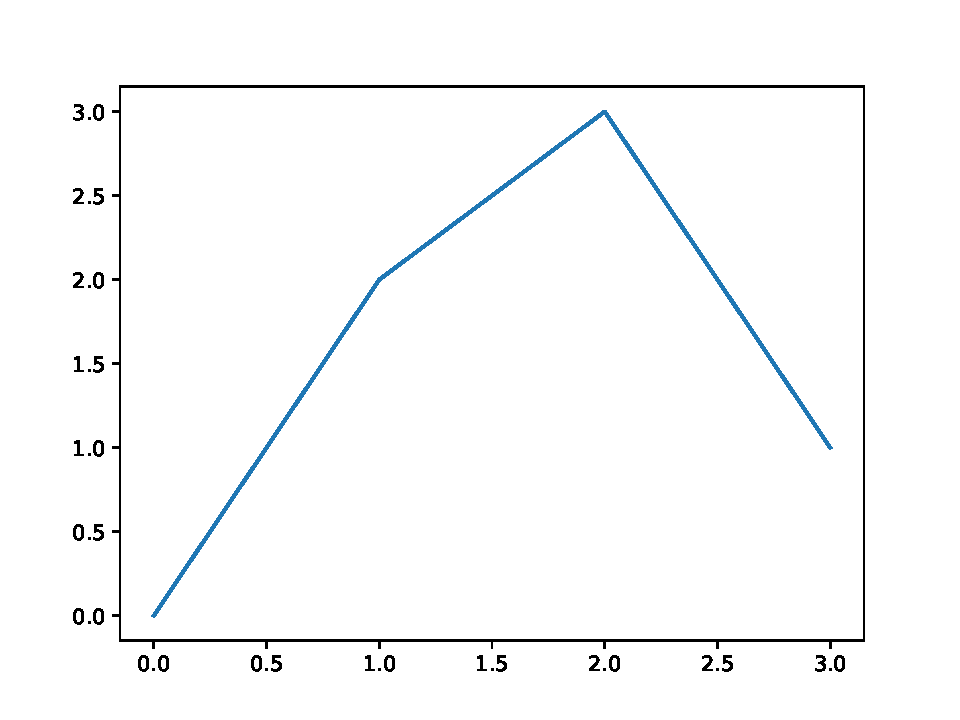
\includegraphics[height=2.5in]{beginning}
  \caption{A simple example}
  \label{fig:beginning}
\end{figure}

\end{document}